%%%%%%%%%%%%%%%%%%%%%%%%%%%%%%%
% Based on template:  wdg-Beamer.tex
%%     A template for using APA citation style in Beamer, with bibLaTeX and biber
%       Uses bibLaTeX and beamer and biber
%%%%%%% does NOT use Brian Beitzel's document class "apa6" for writing documents in APA style
% %%%%%%%%%% does use Philip Kline's apa6 citations for writing citations in APA style
%
% Begun 2012-01jan-18 by w.gray
%%%%%%%%%%%%%%%%%%%%%%%%%%%%%%%%%%

%%%%%%%%%%%%%%%%%%%%%%%%%%%%%%%%%%%%%%%%%%%%%%%%%%%%%
%%%%%%%%%%%%%%%%%% SET UP DOCUMENT - GENERAL STUFF %%%%%%%%%%%%
%%%%%%%%%%%%%%%%%%%%%%%%%%%%%%%%%%%%%%%%%%%%%%%%%%%%%%

\documentclass[usenames,dvipsnames]{beamer}
%% wdg KOOL - I can add options here for packages like xcolor and color that Beamer automatically loads

%%% HOW TO PRODUCE HANDOUTS %%%%%

%%%		beamer modes: handout, 
%%% Removing overlays from a beamer presentation is easily done within the preamble, by adding the handout option:
%\documentclass[handout,xcolor=pdftex,dvipsnames,table]{beamer}
% Once overlays have been removed, putting multiple frames onto a single sheet of paper is a separate problem related to PDF files. The pdfpages package [4], for example, solves this problem. For an automated approach based on the same package, pdfjam [1], a Unix shell script, can be used.

%%% PACKAGES LOADED IN BY BEAMER
%%%		amsthm %%use noamsthm to suppress loading this -- see p16 of beameruserguide (BUG)
%%%		color - also xcolor is loaded
%%%		enumerate %% loaded in the presentation modes but not in the article mode
%%%		hyperref   %% to pass additional options to beamer use the following class options: \documentclass[hyperref={<list-of-options}]{beamer}
%%%		for HANDOUTS recommended that you use beamer with the document class article
	%%% \documentclass[<options>]{article}
	%%%	\usepackage[<options>]{beamerarticle}
	%%%	--- see the BUG for more details, pp206
%%%		xcolor - also color is loaded


\mode<presentation>
%\hypersetup{pdfpagemode=FullScreen} % makes your presentation go automatically to full screen

\usetheme{Madrid}
\usecolortheme{beaver} %crane fly wolverine 

%\useoutertheme[subsection=false]{smoothbars}

\useinnertheme{rectangles}

\setbeamercovered{transparent} %% having this on should make all not-yet-uncovered-text transparent
%% {\setbeamercovered{invisible}{ \begin{frame} . . . \end{frame} }} - as a wrapper to turn off the transparent mode for one frame. Used in my 121011-ONR-SF_rvw presentation for the Just-Manageable-Complexity frame - which has graphics

\setbeamertemplate{navigation symbols}{} %% to eliminate the navigation buttons from bottom of slides
%%%%%%%%%%%%%%%%%%%%%%%%%%%%%%%%%%%%%%%%%%%%
%%%%          EXPERIMENTAL STUFF

%%% for drawing
\usepackage{pgf}
\usepackage{tikz}

%% CONTROL FONT SIZE ON ONE PAGE - 120918
\usepackage{lipsum}

\newcommand\ChangeFontSize{\fontsize{9}{7.2}\selectfont}
\newcommand\ChangeFontSizeVS{\fontsize{8}{7}\selectfont}
%%% USAGE: just put the "\ChangeFontSize" command on a line, by itself, immediately before the items you want to change. Such as before an "\begin{itemize}" command.

\usepackage{units}%% for \nicefrac{1}{2} such as 1/2
\usepackage{textcomp}%% for \textonehalf 

\usepackage{adjustbox}

%%%%%%%%%%%%%%% stuff for my custommade colorboxes for use in references
\newenvironment<>{citeBlock}[1]{%
  \begin{actionenv}#2%
      \def\insertblocktitle{#1}%
      \par%
      \mode<presentation>{%
        \setbeamercolor{block title}{fg=white,bg=orange!20!black}
       \setbeamercolor{block body}{fg=black,bg=gray!20}
       \setbeamercolor{itemize item}{fg=orange!20!black}
       %\setbeamertemplate{itemize item}[triangle]
     }%
      \usebeamertemplate{block begin}}
    {\par\usebeamertemplate{block end}\end{actionenv}}
%%%% USAGE -- use inside a "\begin{textblock}{11.5}(1,13) . . . \end{textblock}" as you would any other block with "\begin{citeBlock}  . . . \end{citeBlock}"

%%%%%%%%%%%%%%%%%%%%%%   END EXPERIMENTAL STUFF   %%%%%%%%%%%%%%%%%%%%%%
%%%%%%%%%%%%%%%%%%%%%%%%%%%%%%%%%%%%%%%%%%%%%%%%%%%%%%%%%%%%%%%%%%

%%%%%%%%%%%%%%%%%%%%%%%%%%%%%%%%%%%%%%%%%%%%%%%%%%%
%%%		OTHER PACKAGES LOADED IN EVERYTIME	%%%%%%%%%%%
%%%%%%%%%%%%%%%%%%%%%%%%%%%%%%%%%%%%%%%%%%%%%%%%%%%%%

\usepackage{graphicx} % Defines \includegraphics*

%\usepackage[latin1]{inputenc} %% commented this out cause I like the default font


%\usepackage{times} %% commented this out cause I like the default font

\usepackage[T1]{fontenc}

\usepackage{pifont} %for dingbat style things such as ARROWS, see the ``symbol-letter guide'' in my Guides folder for LaTeX

% Or whatever. Note that the encoding and the font should match. If T1
% does not look nice, try deleting the line with the fontenc.

\usepackage[absolute,overlay]{textpos}
%%%		beamer automatically installs a white background behind everything, unless you install a different background template. Because of this, you must use the overlay option when using textpos, so that it will place boxes in front of everything. Alternatively, you can install an empty background template, but this may result in an incorrect display in certain situtations with older versions of the Acrobat Reader.

\usepackage{url} % Typeset URLs and e-mail addresses

\usepackage{geometry} %\usepackage{geometry}
%\usepackage{movie15}%\usepackage{movie15}

%\usepackage{multimedia} %% THIS IS MY DEFAULT FOR MOVIES

\usepackage{setspace}  %%% THIS IS USED BY THE SETLENGTH COMMAND, AND OTHER SPACE COMMANDS BELOW

%\usepackage[usenames]{color}

\xdefinecolor{darkgreen}{rgb}{0,0.35,0}
\definecolor{wdgRed}{rgb}{.6,0,0}
\definecolor{gray90}{gray}{0.90}
\definecolor{gray75}{gray}{0.75}
\definecolor{gray50}{gray}{0.50}
\definecolor{LightCyan}{rgb}{0.88,1,1}
%\definecolor{LightCyan}{rgb}{0.88,1,1}


%%%%%%%%%%%%%%%%%%%%%%%%%%%%%%%%%%%%%%%%%%%%%%%%%%%%%
%%%%%%%%%%%%%%%%%% Biblatex APA6 Stuff %%%%%%%%%%%%%%%%%%%%%%%%
%%%%%%%%%%%%%%%%%%%%%%%%%%%%%%%%%%%%%%%%%%%%%%%%%%%%%%
\usepackage[american]{babel}
\usepackage{csquotes}
\usepackage[style=apa,backend=biber]{biblatex}
\DeclareLanguageMapping{american}{american-apa}


%\addbibresource{mini.bib} %%%NAME OF SAMPLE BIB

\addbibresource{/Users/GrayMatter/Library/texmf/tex/wdg_master_Bib.bib} %my default biblatex file

\setlength{\bibhang}{1.5em}  %%% adjusts the hanging indent size

%%% PATHNAME FOR LOGO FIGURES
%% /Users/GrayMatter/Library/texmf/tex/zLogoFigs


\usepackage[yyyymmdd]{datetime}

\usepackage{verbatim}

%%%%%%%%%%%%%%%%%%%%%%%%%%%%%%%%
%%%%	BEAMER SETUPS
%%%%%%%%%%%%%%%%%%%%%%%%%%%%%%%
\AtBeginSection[] % Do nothing for \section*
{
	\begin{frame}<beamer>
		\frametitle{Outline}
		\tableofcontents[currentsection]
	\end{frame}
}

\AtBeginSubsection[]
{
  \begin{frame}<beamer>{Outline}
    \tableofcontents[currentsection,currentsubsection]
  \end{frame}
}

%these commands can make the cell entries ragged right 
%\newcommand{\rr}{\raggedright}
%\newcommand{\tn}{\tabularnewline}

%\titlegraphic{\includegraphics[width=\textwidth,height=.5\textheight]{someimage}}

%%%%%%%%%%%%%%%%%%%%%%%%%%%%%%%%%%%%%%%%%%%%%%%%%%%%%%%%%%
%%%%%%%%%%%%%%%%%% SPECIALS FOR THE TABLE  %%%%%%%%%%%%%%%%%%%%%
%%%%%%%%%%%%%%%%%%%%%%%%%%%%%%%%%%%%%%%%%%%%%%%%%%%%%%%%%%

%%\usepackage{tabu} - clashes with some other packages
\usepackage{colortbl} %% colored lines in tables
%% to "easily" allow us to make the first row of a table BOLD font
%%% see: http://www.tex.ac.uk/cgi-bin/texfaq2html?label=wholerow
\newcolumntype{$}{>{\global\let\currentrowstyle\relax}}
\newcolumntype{^}{>{\currentrowstyle}}
\newcommand{\rowstyle}[1]{\gdef\currentrowstyle{#1}%
  #1\ignorespaces
}

%%%%%%%%%%%%%%%%%%%%%%%%%%%%%%%%%%%%%%%%%%%%%%%%%%%%%%%%%
%%%%   LOGO - setups, macro for turning off, and instructions for off/on %%%%
%%%%%%%%%%%%%%%%%%%%%%%%%%%%%%%%%%%%%%%%%%%%%%%%%%%%%%%%%

% If you have a file called "university-logo-filename.xxx", where xxx
% is a graphic format that can be processed by latex or pdflatex,
% resp., then you can add a logo as follows:

\pgfdeclareimage[height=1cm]{university-logo}
{/Users/GrayMatter/Library/texmf/tex/zLogoFigs/CWL-s.pdf} %[height=0.5cm]
\logo{\pgfuseimage{university-logo}}

%%% LOGO OFF/ON
\newcommand{\nologo}{\setbeamertemplate{logo}{}} % command to set the logo to nothing
% must enclose the frame(s) without the logo in braces
% any number of frames can be within the group.

%%%% USAGE
\begin{comment}
  {\nologo
	\begin{frame}\frametitle{Test frame no logo}
	\end{frame}
	\begin{frame}\frametitle{Another Test frame no logo}
	\end{frame}
  }
\end{comment}
%%%%%%%%%%                    END LOGO SECTION                   %%%%%%%%%%%%%%

% If you wish to uncover everything in a step-wise fashion, uncomment
% the following command: 

%\beamerdefaultoverlayspecification{<+->}

%%%%%%%%%%%%%%%%%%%%%%%%%%%%%%%%%%%%%%%%%%%%%%%%%%%%%
%%%%%%%%%%%%%%%%%% Title Page Info %%%%%%%%%%%%%%%%%%%%%%%%%%%
%%%%%%%%%%%%%%%%%%%%%%%%%%%%%%%%%%%%%%%%%%%%%%%%%%%%%%

\title[Inside Models] % (optional, use only with long paper titles)
{Models, Modeling, and Muddles}

%\subtitle{Eye Data in Immediate Interactive Behavior}

\author[W. D. Gray]%
{Wayne D. Gray} % (optional, use only with lots of authors)
% - Give the names in the same order as the appear in the paper.
% - Use the \inst{?} command only if the authors have different affiliations.

\institute[Rensselaer] % (optional, but mostly needed)
{Cognitive Science Department, Rensselaer Polytechnic Institute}

% - Use the \inst command only if there are several affiliations.
% - Keep it simple, no one is interested in your street address.

\date[\today] % (optional, should be abbreviation of conference name)
{Talk Presented at the 56th Annual Meeting of the Human Factors \& Ergonomics Society\\2012-October-24}
% - Either use conference name or its abbreviation.
% - Not really informative to the audience, more for people (including yourself) who are reading the slides online

%\subject{<>}
% This is only inserted into the PDF information catalog. Can be left
% out. 

%%%%%%%%%%%%%%%%%%%%%%%%%%%%%%%%%%%%%%%%%%%%%%%%%%%%%
%%%%%%%%%%%%%%%%%% BEGIN DOCUMENT HERE  %%%%%%%%%%%%%%%%%%%%%
%%%%%%%%%%%%%%%%%%%%%%%%%%%%%%%%%%%%%%%%%%%%%%%%%%%%%%

\begin{document}

\begin{frame}
  \titlepage

\end{frame}

\section{Sheridan's Taxonomy}

\begin{frame}
	\frametitle{SHERIDAN'S TAXONOMY OF MODEL ATTRIBUTES}

	\begin{center}
	\resizebox{\textwidth}{!}{
	\begin{tabular}{l| $>{\centering\arraybackslash}m{3cm} |$>{\centering\arraybackslash}m{3cm}|$>{\centering\arraybackslash}m{3cm}|$>{\centering\arraybackslash}m{3cm}}
	\hline \rowcolor{gray50}
	&	\textcolor{white}{ATTRIBUTE}		&	\textcolor{white}{1 (LEAST)}	&	\textcolor{white}{2 (MODERATE)}	&	\textcolor{white}{3 (MOST)}\\
\hline
\rowcolor{gray75}
	A    &	DATA APPLICABILITY	&	No basis in existing data	&	Describes existing data	&	Predicts future data\\
\hline 	\rowcolor{gray90}
	B    & DIMENSIONALITY		&	Single input, single output	& Multi input, single output	& Multi input, multi output\\
\hline
\rowcolor{gray75}
	C   &	METRICITY				& Limited to nominal relationships & Primarily ordinal relationships & Entirely cardinal relationships\\
\hline \rowcolor{gray90}
	D   &	ROBUSTNESS			&	Unique focus on limited objects or events & Moderate focus to a variety of objects or events	&	Comprehensive of a wide slice of nature\\
\hline
\rowcolor{gray75}
      E    &	SOCIAL PENETRATION		&	Confined to a mental model	&	Communicated to the relevant community	&	Accepted and used by the relevant community\\

	\end{tabular}
}
	\end{center}
\end{frame}



\section{Models Presented at HFES}
\subsection{Predicting Task Duration \& Variability}

%% undoes the effect of \setbeamercovered{transparent} used in the prolog
{\setbeamercovered{invisible}{
\begin{frame}
	\frametitle{Tools for Predicting the Duration and Variability of Skilled Performance without 
Skilled Performers - HFES12 - Thur 8:00 HP2}
	\vspace{-4.2cm}
	SANLab Models (Stochastic Analytic Network Laboratory)
	\begin{textblock}{12}(1,5)
		\uncover<1->{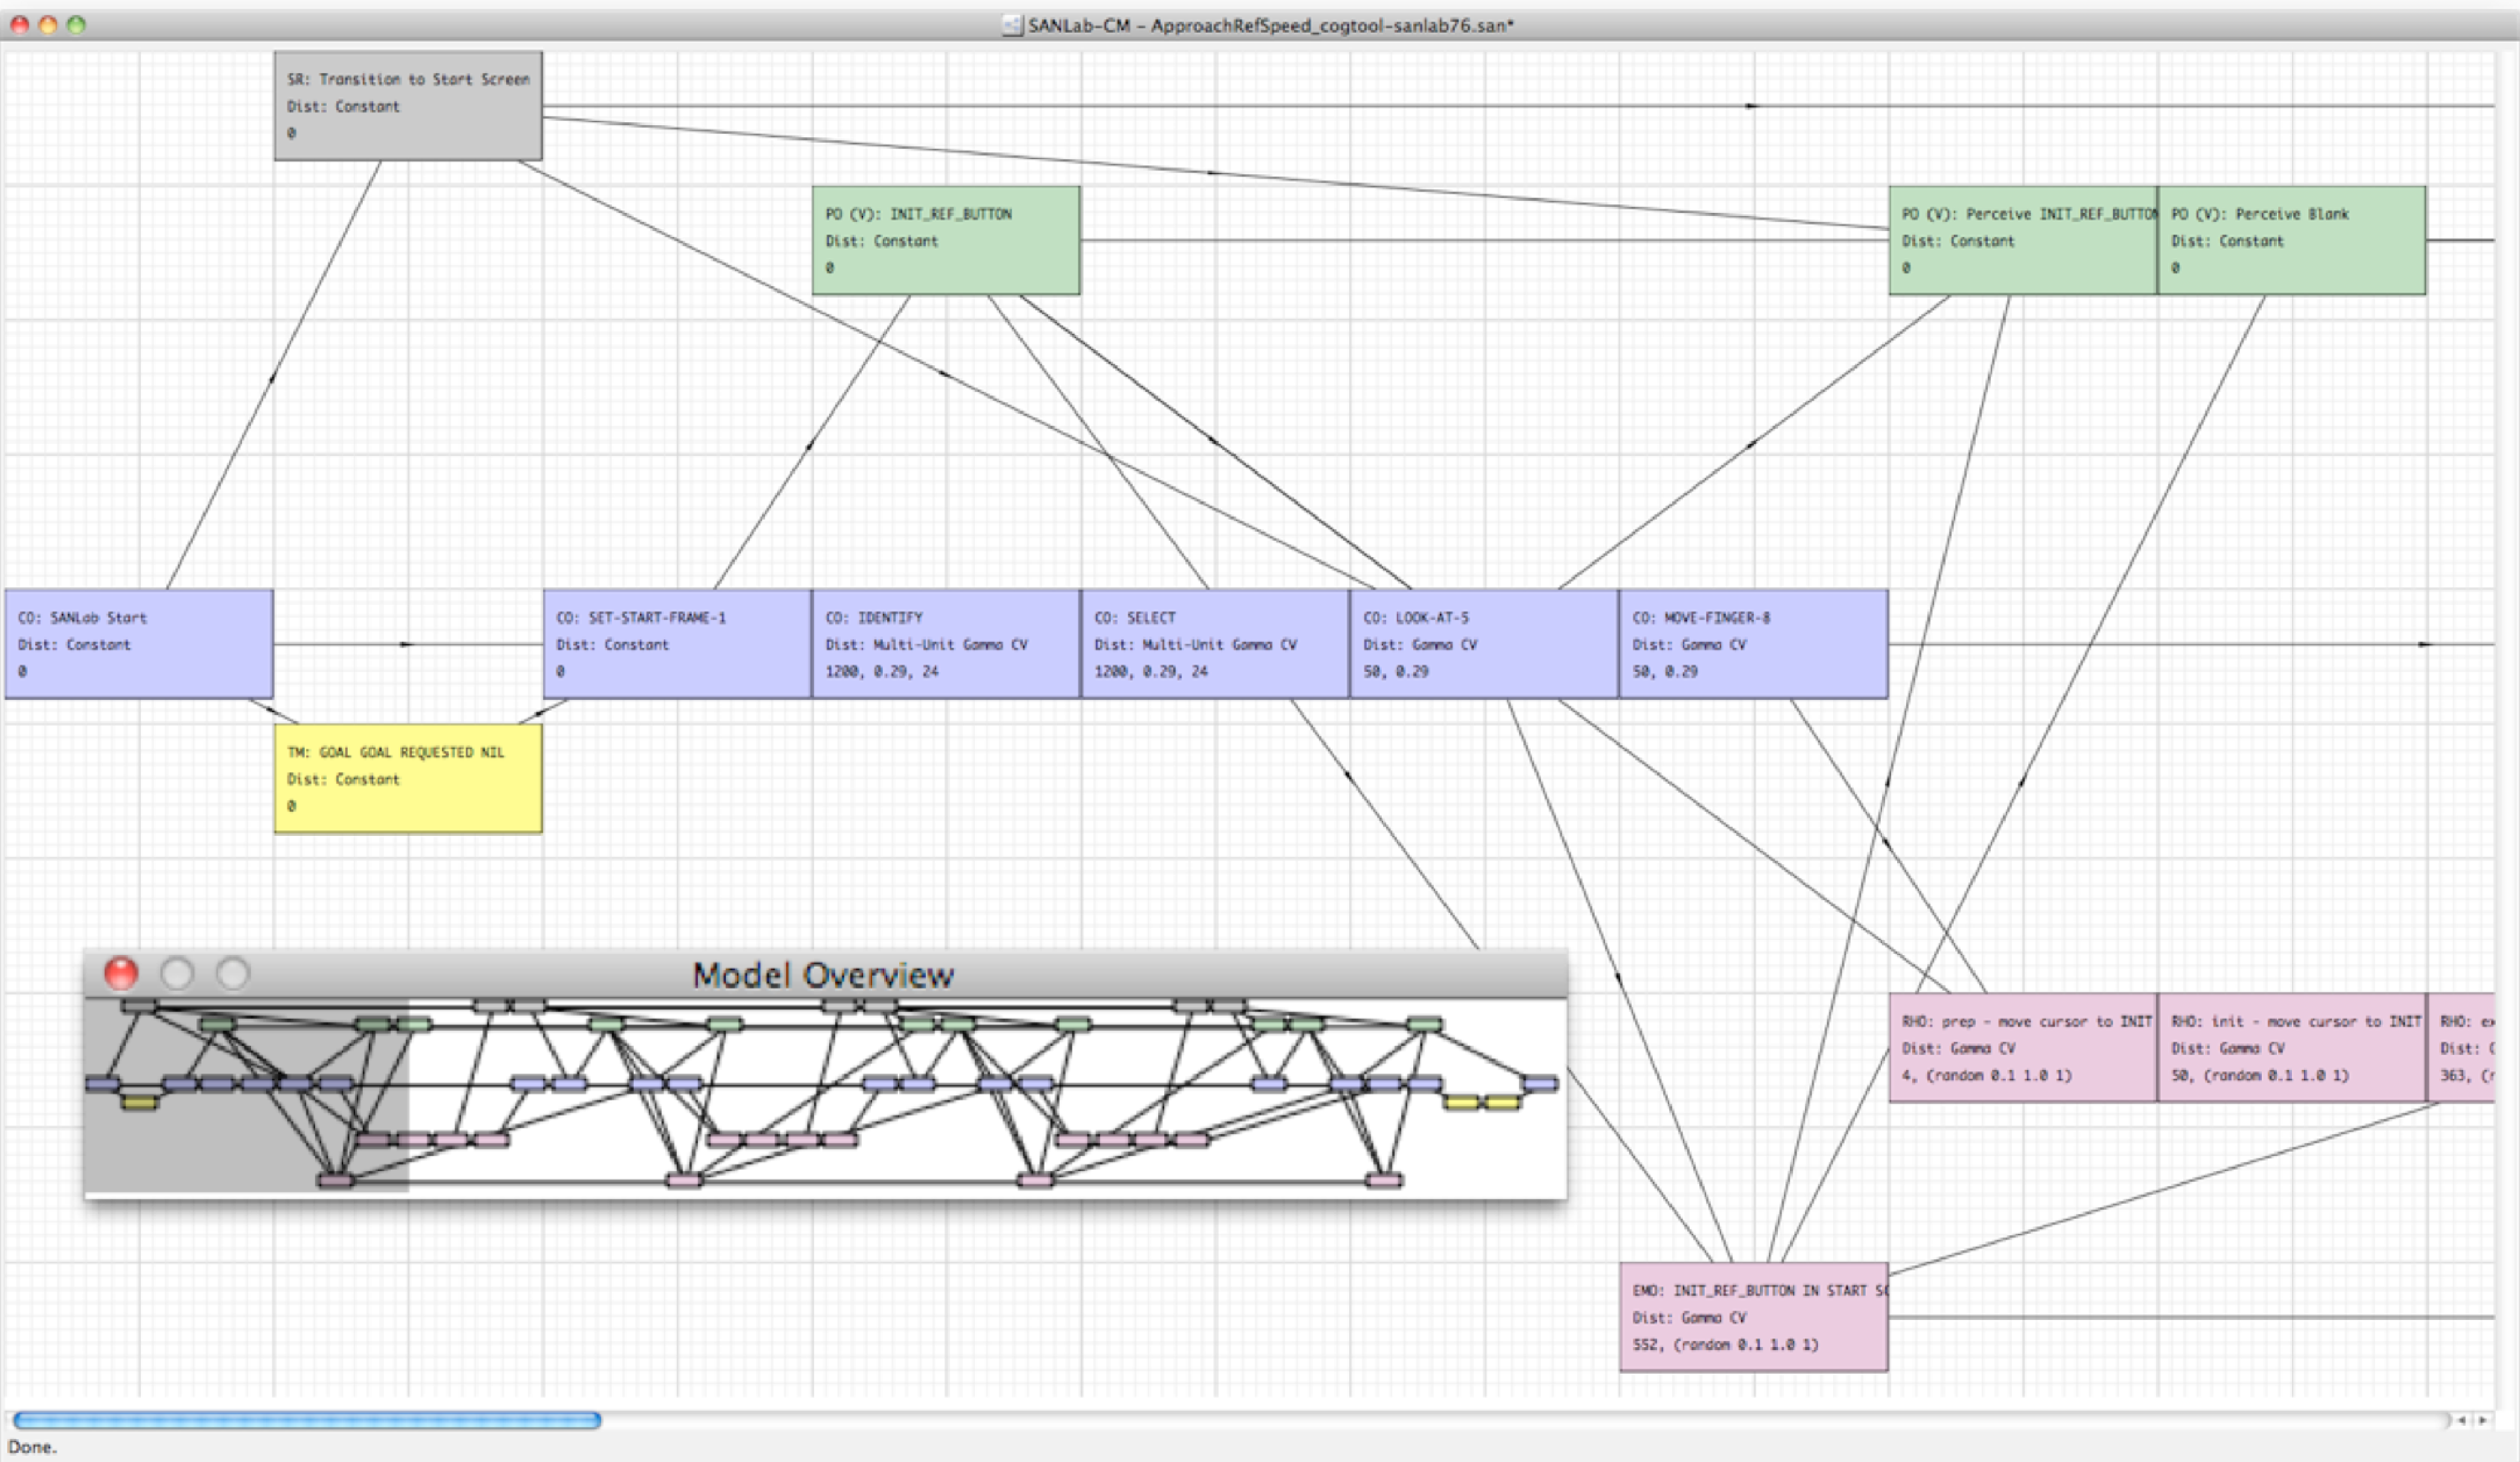
\includegraphics[width=\textwidth]{zFigs/fig4-SL}}
	\end{textblock}
	
	\begin{textblock}{6}(6,7)
		\uncover<2>{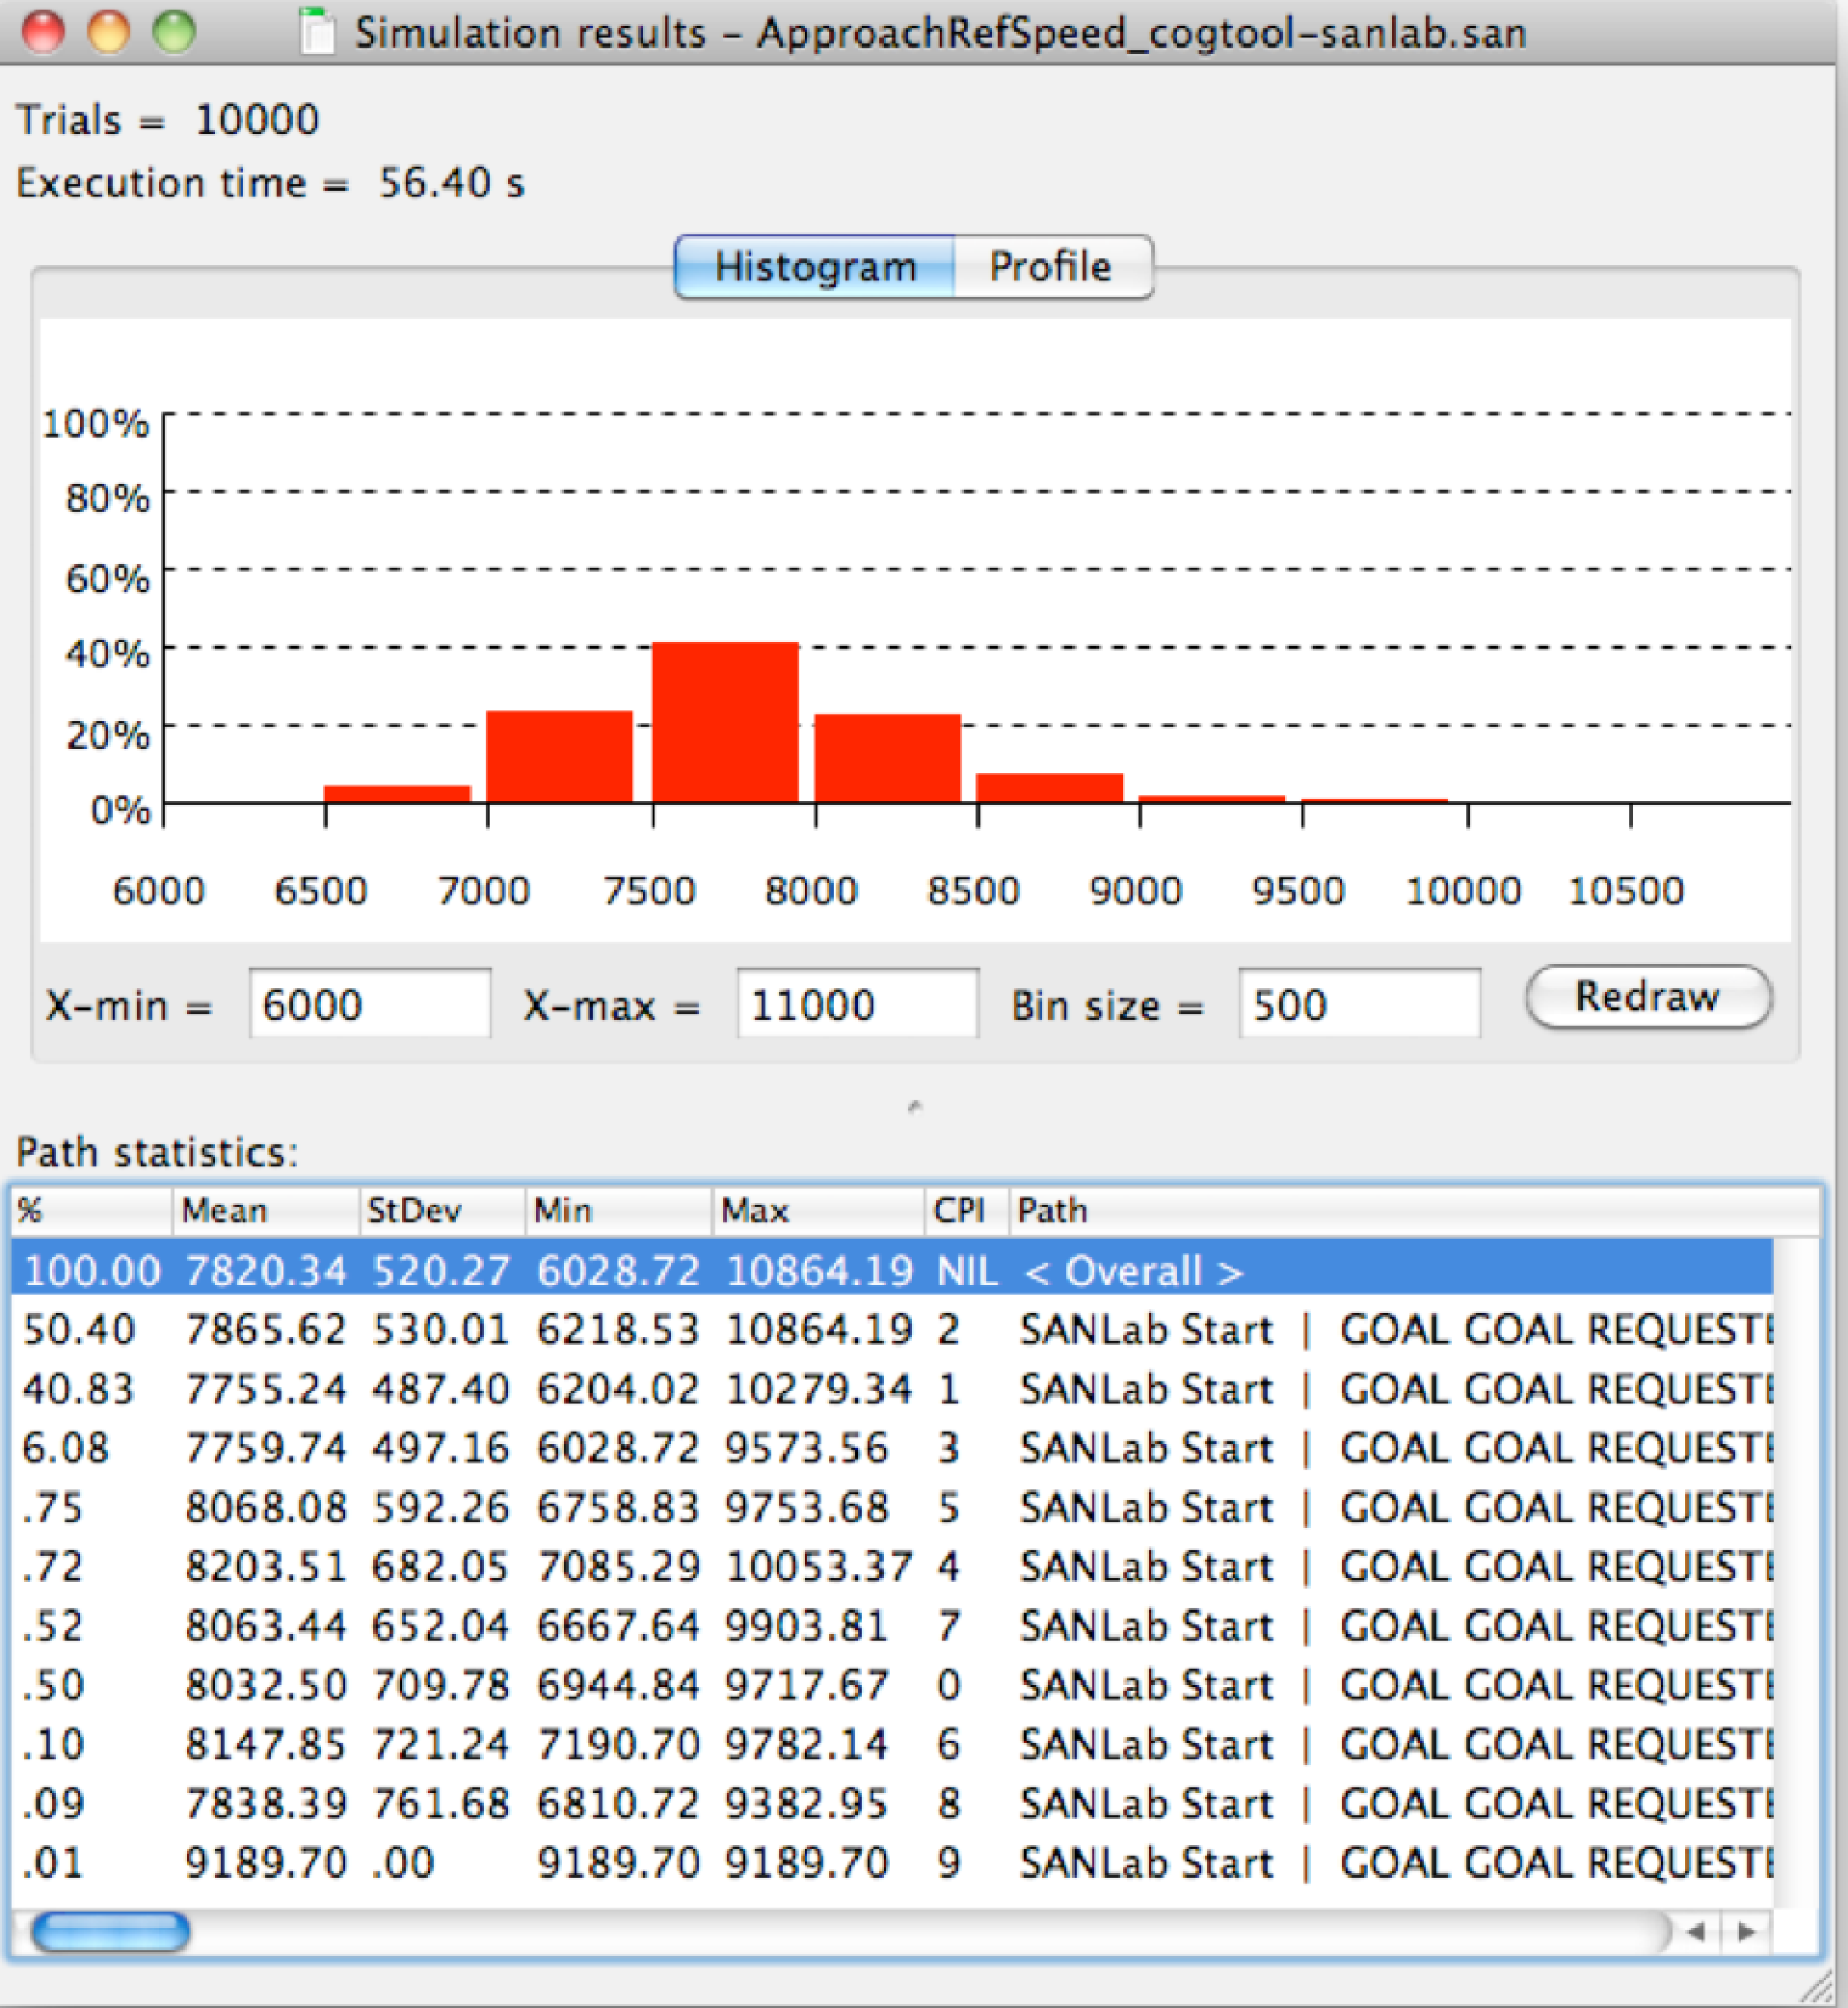
\includegraphics[width=\textwidth]{zFigs/fig5-SLhist}}
	\end{textblock}
\end{frame}
}}

{\nologo{
\begin{frame}
	\frametitle{Tools for Predicting the Duration and Variability of Skilled Performance without Skilled Performers}
	\vspace{-1cm}

	\resizebox{\textwidth}{!}{
	\begin{tabular}{l| $>{\centering\arraybackslash}m{2.7cm} |$>{\centering\arraybackslash}m{3cm}|$>{\centering\arraybackslash}m{6.5cm}}								\hline\rowcolor{gray50}
	&	\textcolor{white}{ATTRIBUTE}		&	\textcolor{white}{CATEGORY (1, 2, or 3)}	&	\textcolor{white}{DISCUSSION}												\\\hline\rowcolor{gray75}
	A    &	\small{DATA APPLICABILITY}			&	3 - Predicts future data			&	Predicts expert performance times and variability w/o experts																	\\ \hline 	\rowcolor{gray90}
	B    & \small{DIMENSIONALITY}				&	3 - Multi input/output			&	Uses \textcolor{wdgRed}{\emph{fixed sets of population parameters}} and task analysis as input. Predicts time + variability for the average person.									\\\hline\rowcolor{gray75}
	C   &	\small{METRICITY	}					&	3 - Cardinal						&	Mean times and Standard Deviations																\\\hline\rowcolor{gray90}
	D   &	\small{ROBUSTNESS}					&	1 - Unique focus (??)				 &	Any one model \alert{should} focus on one design; however, trivial to make multiple models for same or different device 							\\ \hline\rowcolor{gray75}
      E    &	\small{SOCIAL PENETRATION}			&	2-3								&	CogTool is widely used by the interface design community. SANLab is based on Activity Networks which are the formalism underlying CPM-GOMS models as well as MANPRINT, etc													\\
	\end{tabular}
}
	\begin{textblock}{12}(1,13.5)
		\begin{citeBlock}{}
			\tiny{\fullcite{bej12hfes}}
		\end{citeBlock}
	\end{textblock}
\end{frame}
}}

\subsection{Cognitive Workload from EEG}

\begin{frame}
	\frametitle{Cross-subject workload classification with a Hierarchical Bayes Model - HFES11}
	\begin{textblock}{12}(1,4)
		\uncover<1->{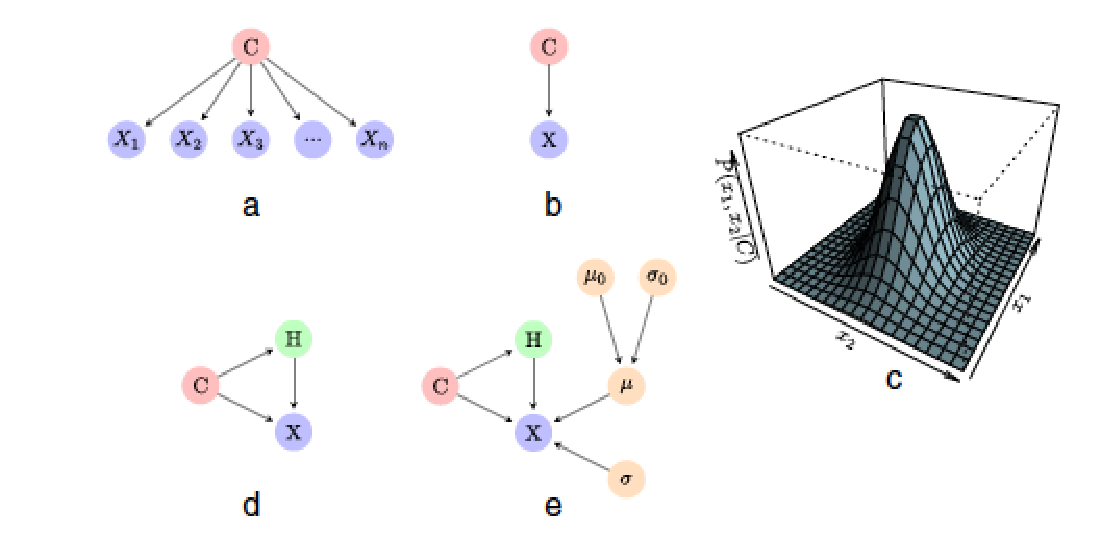
\includegraphics[width=\textwidth]{zFigs/fig1_NeuroImage}}
	\end{textblock}
	\begin{textblock}{12}(1,13)
		\begin{citeBlock}{}
			\tiny{\fullcite{wang12neuroImage}}
		\end{citeBlock}
	\end{textblock}
\end{frame}

{\nologo{
\begin{frame}
	\frametitle{Cross-subject workload classification}
	%\vspace{-1cm}
	Using a non-cognitive, Hierarchical Bayes Model
	\resizebox{\textwidth}{!}{
	\begin{tabular}{l| $>{\centering\arraybackslash}m{2.7cm} |$>{\centering\arraybackslash}m{3cm}|$>{\centering\arraybackslash}m{6.5cm}}								\hline\rowcolor{gray50}
	&	\textcolor{white}{ATTRIBUTE}		&	\textcolor{white}{CATEGORY (1, 2, or 3)}	&	\textcolor{white}{DISCUSSION}												\\\hline\rowcolor{gray75}
	A    &	\small{DATA APPLICABILITY}			&	3 - Predicts future data			&	Uses a training set of multiple people to derive parameters that can read each of their EEG data to recognize their current workload state \textcolor{wdgRed}{(caution - this gloss may make the model sound better than it actually is)}																	\\ \hline 	\rowcolor{gray90}
	B    & \small{DIMENSIONALITY}				&	2 - Multi input/ single output			&	Takes 64 channel EEG data and predicts one CWL measure																	\\\hline\rowcolor{gray75}
	C   &	\small{METRICITY	}					&	2 - Ordinal						&	High, medium, or low workload																\\\hline\rowcolor{gray90}
	D   &	\small{ROBUSTNESS}					&	1 - Unique focus (??)				 &	Workload!!! 							\\ \hline\rowcolor{gray75}
      E    &	\small{SOCIAL PENETRATION}			&	1-3								&	Hierarchical Bayes Analyses are well-accepted in the academic engineering community, apparently new to Human Factors													\\
	\end{tabular}
}
\end{frame}
}}

\subsection{Strategy Evaluation via Cognitive Modeling}

%% undoes the effect of \setbeamercovered{transparent} used in the prolog

\begin{frame}
	\frametitle{Strategy Evaluation via Cognitive Modeling - HFES02}
	\begin{textblock}{12}(1,1.8)
		\uncover<1->{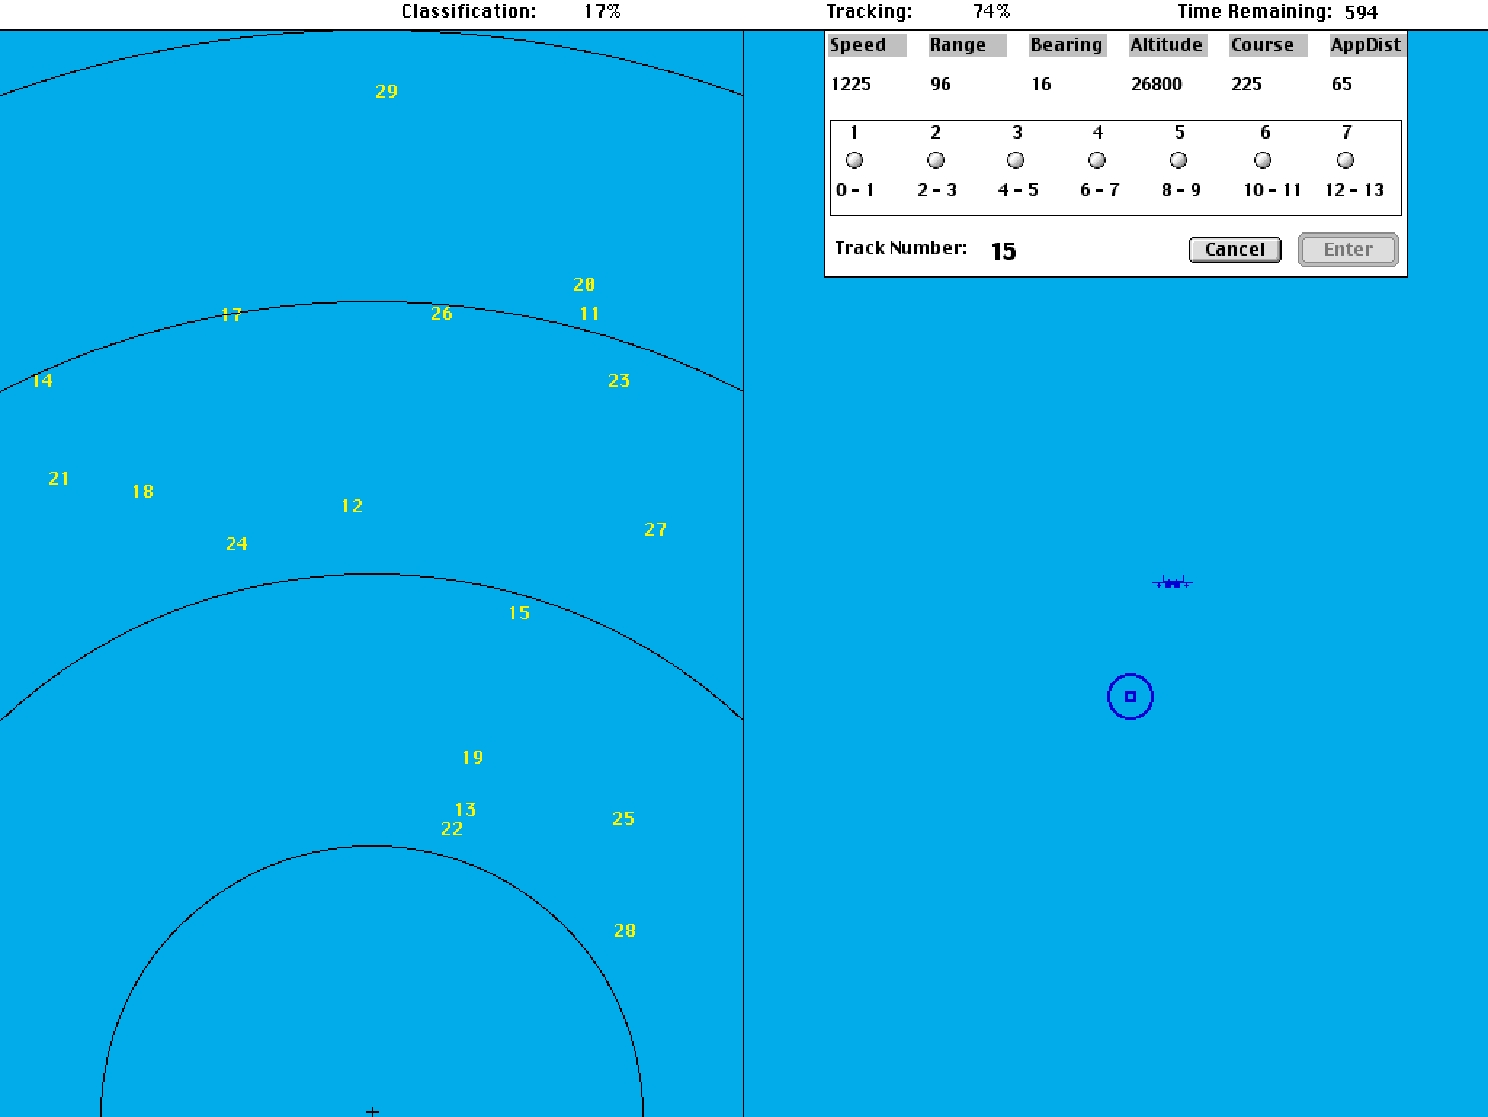
\includegraphics[width=\textwidth]{zFigs/Argus_scr-shot_color}}
	\end{textblock}
	\begin{textblock}{13}(0.8,13.3)
		\begin{citeBlock}{}
			\tiny{\fullcite{gray02hfes}}
		\end{citeBlock}
	\end{textblock}
\end{frame}

{\nologo{
\begin{frame}
	\frametitle{Strategy Evaluation via Cognitive Modeling}
	\vspace{-0.5cm}
	\small{Using a cognitively valid, ACT-R model locked into one of 3 search strategies -- asking a variant of the \textcolor{wdgRed}{\emph{optimality} question} - how useful are the strategies that the researchers \emph{think} they have identified in actually doing the task in question????}\\
\textcolor{white}{extraline}\\

	\resizebox{\textwidth}{!}{
	\begin{tabular}{l| $>{\centering\arraybackslash}m{2.7cm} |$>{\centering\arraybackslash}m{3cm}|$>{\centering\arraybackslash}m{6.5cm}}								\hline\rowcolor{gray50}
	&	\textcolor{white}{ATTRIBUTE}		&	\textcolor{white}{CATEGORY (1, 2, or 3)}	&	\textcolor{white}{DISCUSSION}												\\\hline\rowcolor{gray75}
	A    &	\small{DATA APPLICABILITY}			&	??? none of these categories really fit			&	Eliminates possible interpretations, does not necessarily describe the data																	\\ \hline 	\rowcolor{gray90}
	B    & \small{DIMENSIONALITY}				&	2 - Multi input/ single output			&	Takes hours of observation and data analyses to derive 3 candidate strategies, then tries to find the one that matches human achievement																	\\\hline\rowcolor{gray75}
	C   &	\small{METRICITY	}					&	??? not sure this is the right metric for this research question						&  Issue is whether performance using any of the candidate strategies come close to matching human performance  \\\hline\rowcolor{gray90}
	D   &	\small{ROBUSTNESS}					&	1 - Unique focus (??)				 &	What the heck are our subjects doing???? 							\\ \hline\rowcolor{gray75}
      E    &	\small{SOCIAL PENETRATION}			&	1-3								&	Do any of the strategies suggested by \emph{observation} come anywhere close to explaining the data??								\\
	\end{tabular}
}
\end{frame}
}}

\section{Other Visions}
\begin{frame}[label=sampleAgainframe]
	\frametitle{OTHER VISIONS OF MODELS: \emph{McClelland, 2009}}
	``The essential purpose of cognitive modeling is to allow investigation of the implications of ideas, beyond the limits of human thinking.
	\begin{itemize}[<+->]
		\item Models allow the exploration of the implications of ideas that cannot be fully explored by thought alone.
		\item As such, they are vehicles for scientific discovery, in much the same way as experiments on human (or other) participants. 
		\item But the discoveries take a particular form: A system with a particular set of specified properties has another set of properties that arise from those in the specified set as consequences.
		\item From observations of this type, we then attempt to draw implications for the nature of human cognition'' \parencite{mcclelland09topiCS}
	\end{itemize}

	\begin{textblock}{8}(1,13)
		\begin{citeBlock}{}
			\tiny{\fullcite{mcclelland09topiCS}}
		\end{citeBlock}
	\end{textblock}
\end{frame}

\begin{frame}
	\frametitle{IMPORTANCE OF SIMPLIFICATION -- from McClelland, 2009}
	\begin{itemize}[<+->]
		\item ``\textcite{borges98exactitude} describes a town where there are mapmakers who are obsessed with verisimilitude in their mapmaking
		\begin{itemize}
			\item Each strives to outdo the others in making his maps more detailed and realistic. Some mapmakers are criticized because their maps are too small--their scale prevents recording of many details. Others are criticized for schematic rendering of roads and intersections.
			\item The consequence is the construction of huge, life-size maps, which, of course, are completely useless because use of such a map is no easier than direct exploration of the real space that the map represents.
		\end{itemize}
		\item When it comes to mapmaking, simplification is evidently crucial--the point of the map is to offer a guide, rather than a replication, of reality.''
	\end{itemize}

	\begin{textblock}{8}(1,13.5)
		\begin{citeBlock}{}
			\tiny{\fullcite{borges98exactitude}}
		\end{citeBlock}
	\end{textblock}
\end{frame}

\begin{frame}
	\frametitle{MORE MCCLELLAND}
The point is simply this: 
	\begin{itemize} 
		\item Simplification is essential, but it comes at a cost, and real understanding
depends in part on understanding the effects of the simplification. 
		\item Unfortunately, this can mean that further exploration becomes more technical and complex as a result.
			\item Trying hard to add just enough additional complexity can help. Learning what simplification is the best one to use is also a part of the process. Some simplifications do a better job retaining essential properties of a process than others.
	\end{itemize}
\end{frame}

\begin{frame}
	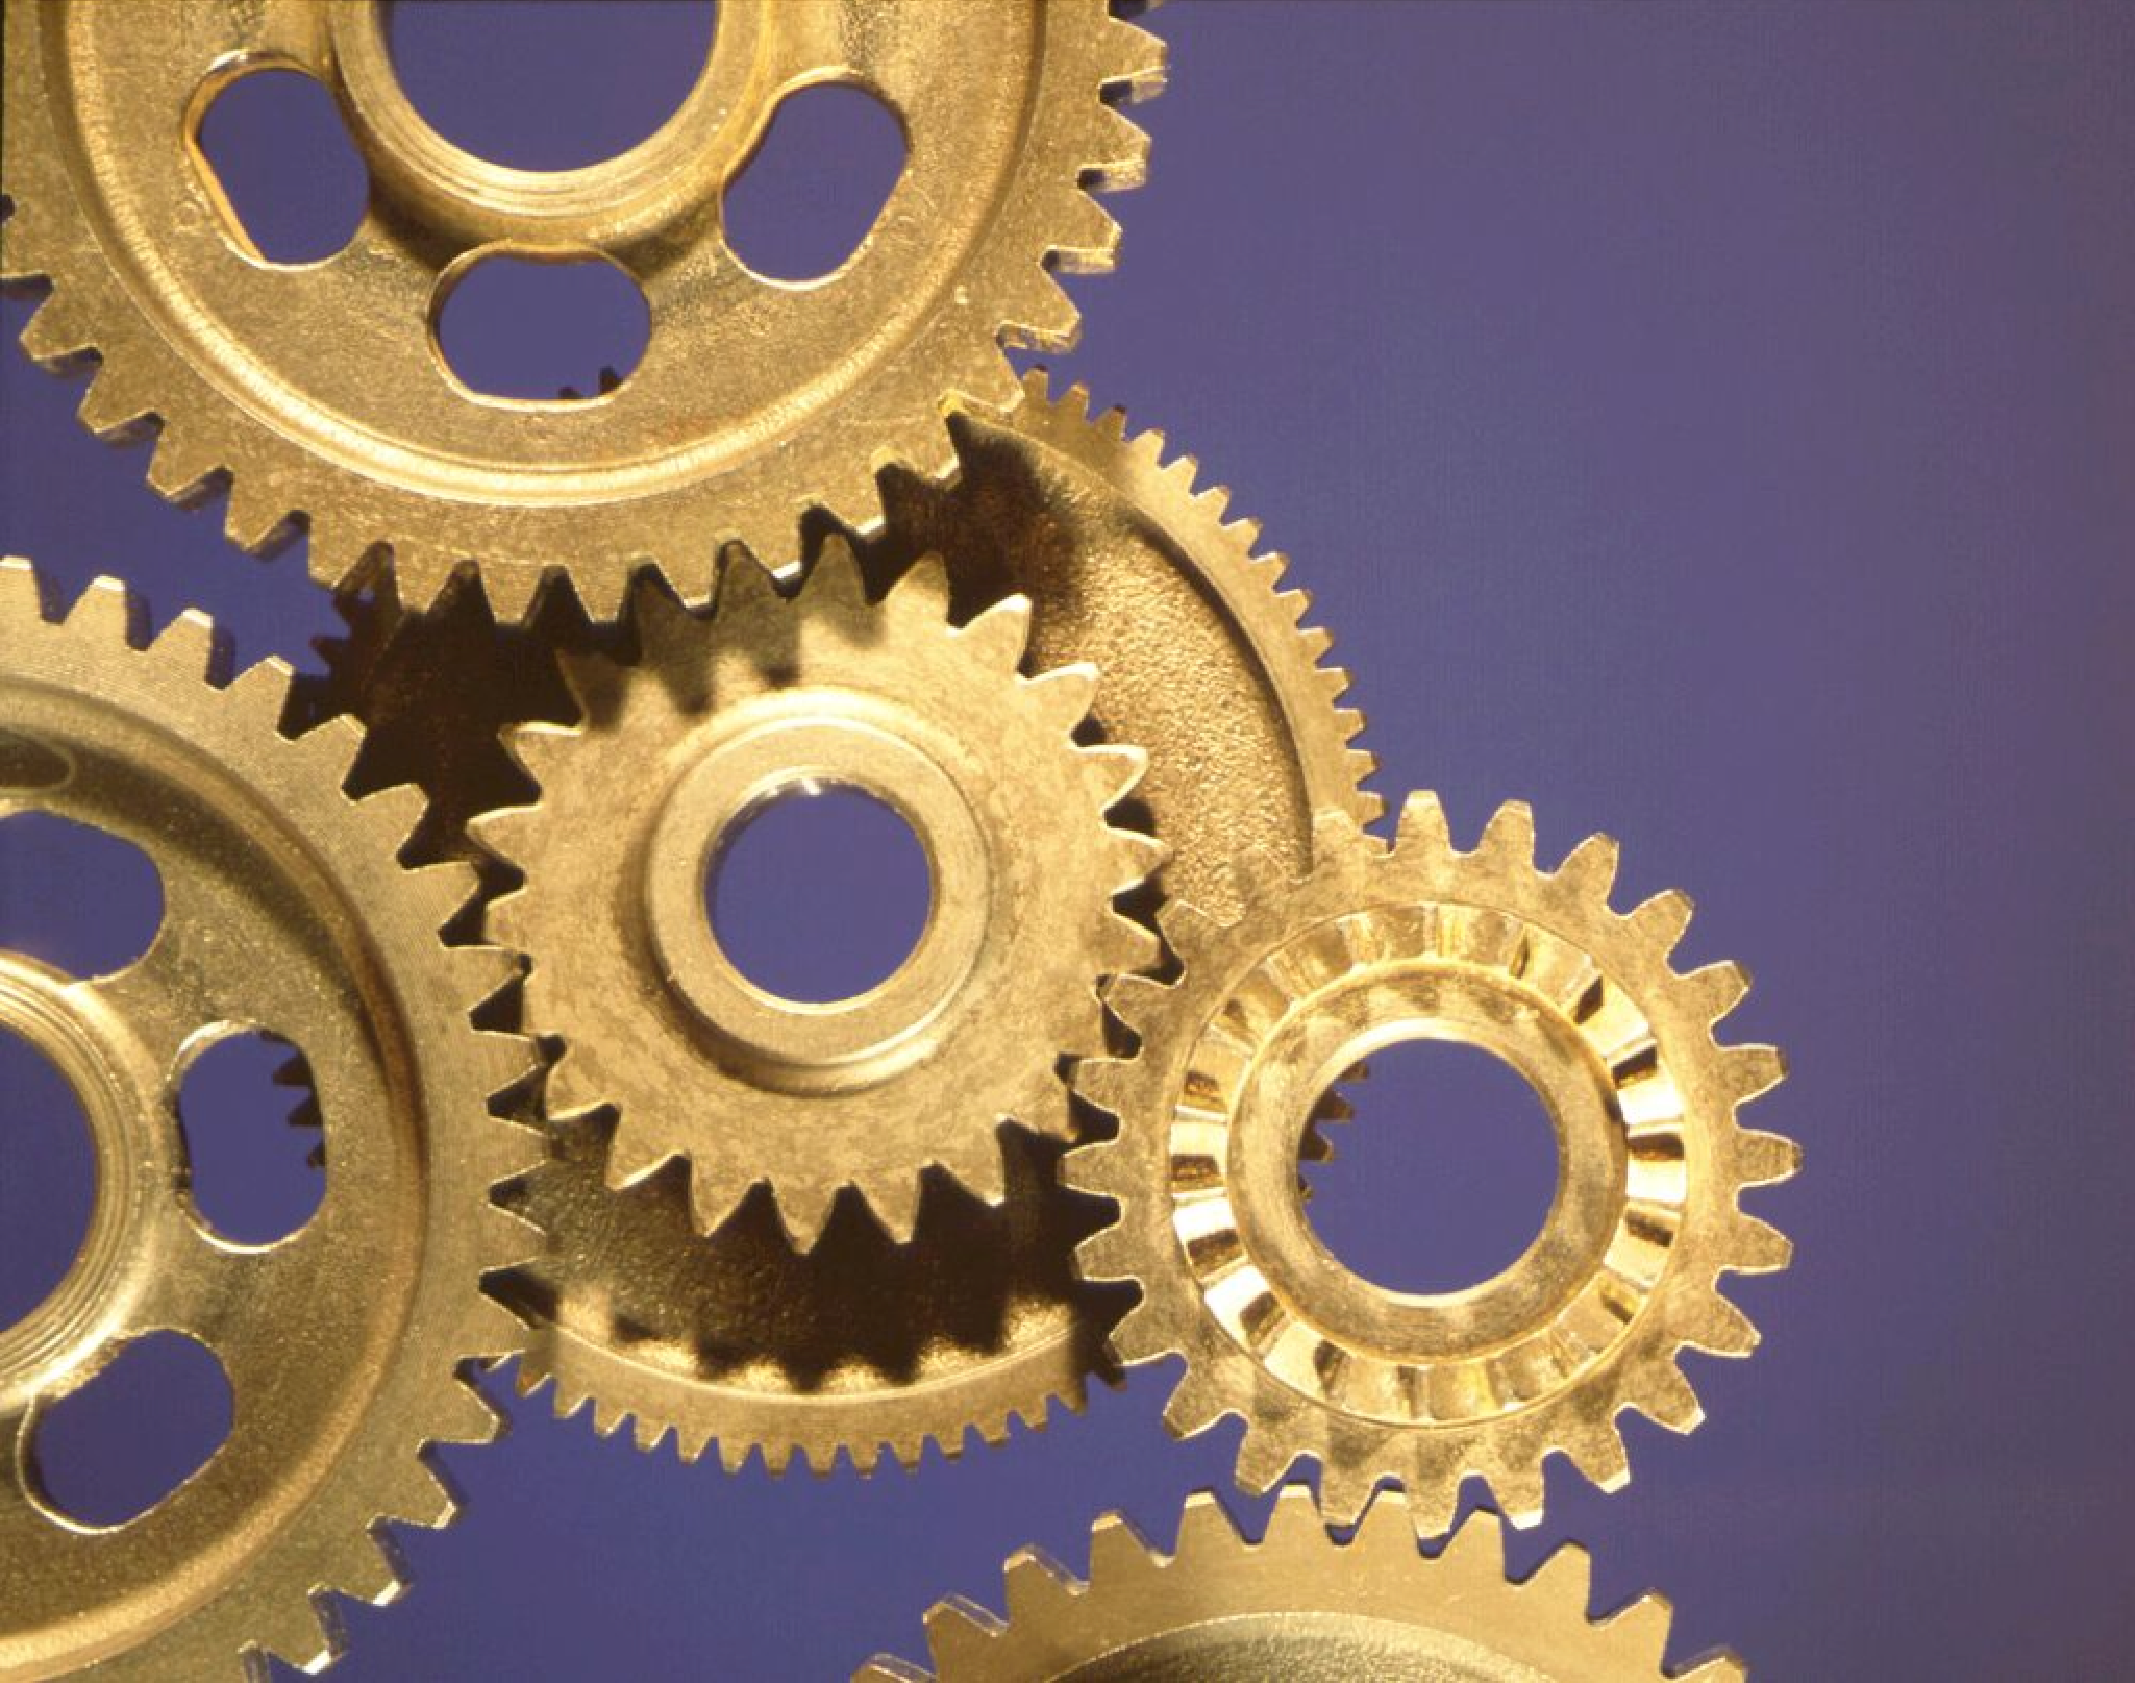
\includegraphics[width=\linewidth]{zFigs/cogWheels}
	\begin{textblock}{4}(11,7)
		\LARGE{\textcolor{wdgRed}{Thank You!!}}
	\end{textblock}
		
	%\begin{textblock}{5}(10,3)
	%	\LARGE{\textcolor{wdgRed}{Haben Sie vielen Dank!}}
	%\end{textblock}
\end{frame}

\end{document}


